% Fig 2.11 / spec Fig A06 -- the interval probability is the area under the
% density curve.  Source: mathstatch2.tex lines 707-739.
% Per spec 1.6 the schematic curve 2 e^{-(t-3)^2/2} is replaced by the true
% N(3,1) density f(t) = 0.3989423 e^{-(t-3)^2/2}, which integrates to 1.
% Drawing scale x=1.15cm, y=8.74cm; peak f(3) = 0.3989423 -> 3.4868cm.
% Shaded region: [a, b] with a = 1.6 and b = 4.8 (the spec moves b from 4.4
% to 4.8 so that the interval is not symmetric about the mode).
\documentclass[tikz,border=2pt]{standalone}
\usepackage{amsmath}
\usepackage{amssymb}
\usepackage{xcolor}
\usetikzlibrary{arrows.meta}
\newcommand{\sssig}{\scriptscriptstyle}

\definecolor{journalink}{HTML}{1F1C18}
\definecolor{journalmuted}{HTML}{8A7F72}
\definecolor{journalaccent}{HTML}{9C2D2D}

\begin{document}
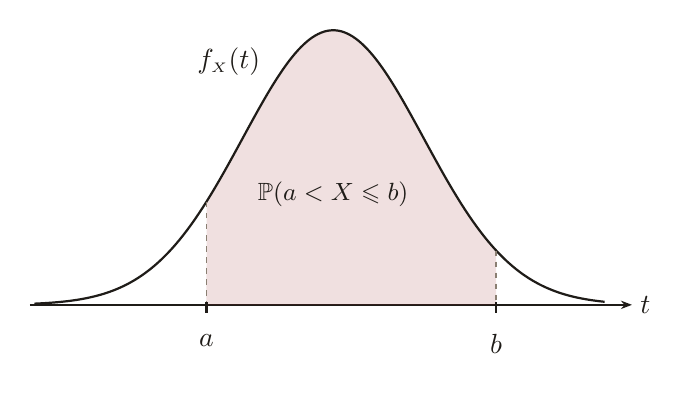
\begin{tikzpicture}[
  x=1.15cm,
  y=8.74cm,
  every node/.style={font=\normalsize, journalink},
  axis/.style={journalink, line width=0.8pt, -{Stealth[length=4pt]}},
  tick/.style={journalink, line width=0.8pt},
  curve/.style={journalink, line width=0.8pt},
  guide/.style={journalmuted, line width=0.5pt, dash pattern=on 2pt off 2pt},
  region/.style={journalaccent, fill opacity=0.15}
]
  % ---- common bounding box, identical in all four figures of this group ----
  \path (-0.43cm,-0.78cm) rectangle (7.58cm,3.52cm);

  % ---- x axis ----
  \draw[axis] (-0.35,0) -- (6.3,0);

  % ---- shaded area over [a, b] = [1.6, 4.8] ----
  \fill[region]
    (1.6,0) -- (4.8,0) -- (4.8,0.0789502)
    -- plot[domain=4.8:1.6, samples=200, smooth]
       (\x,{0.3989423*exp(-(\x-3)*(\x-3)/2)})
    -- cycle;

  % ---- density curve: N(3,1) ----
  \draw[curve] plot[domain=-0.3:6, samples=200, smooth]
    (\x,{0.3989423*exp(-(\x-3)*(\x-3)/2)});

  % ---- the two boundaries ----
  \draw[guide] (1.6,0.1497275) -- (1.6,0);
  \draw[guide] (4.8,0.0789502) -- (4.8,0);
  \draw[tick] ([yshift=0.035cm]1.6,0) -- ([yshift=-0.106cm]1.6,0);
  \draw[tick] ([yshift=0.035cm]4.8,0) -- ([yshift=-0.106cm]4.8,0);
  \node[anchor=north] at ([yshift=-0.25cm]1.6,0) {$a$};
  \node[anchor=north] at ([yshift=-0.25cm]4.8,0) {$b$};

  % ---- label inside the shaded area ----
  % Centred on the shaded region as it is at the label's own height, not on
  % the midpoint of [a,b].  At yshift 1.40cm the height is 1.40/8.74 = 0.16018;
  % the curve exceeds that for x in [1.649, 4.351], and both a = 1.6 and
  % b = 4.8 fall outside that span, so at this height both edges of the region
  % are the curve itself and the slice is centred on the mode, x = 3.
  % (was 3.2, the midpoint of [a,b], which reads 0.2 too far right.)
  \node[inner sep=0pt] at ([yshift=1.40cm]3.0,0)
    {\small $\mathbb{P}(a<X\leqslant b)$};

  % ---- labels ----
  \node[anchor=south east, inner sep=0pt] at ([yshift=0.38cm]2.2,0.2896916)
    {$f_{\sssig X}(t)$};
  \node[anchor=west, inner sep=2.8pt] at (6.3,0) {$t$};
\end{tikzpicture}
\end{document}
